% Guard: macros.tex is \input both by main.tex (after the packages it needs,
% e.g. amsmath for \DeclareMathOperator) and by individual section files so
% they remain compilable on their own. Loading it twice would redefine every
% \newcommand and abort, so the second and later loads are no-ops.
\ifdefined\PQRmacrosloaded\endinput\fi
\let\PQRmacrosloaded\relax

% --- 0. revision marking ---
% Text added to Section 2 during the current revision is wrapped in \added{...}
% so the advisors can see at a glance what is new. Redefine to \relax to print
% the paper without the marking.
\newcommand{\added}[1]{\textcolor{blue}{#1}}
\long\def\added#1{\begingroup\color{blue}#1\endgroup}  % \long: may span paragraphs


% --- A. operator-style score and function names ---
\newcommand{\HD}{\mathit{HD}}                        % histogram distance; use \HD_\gamma
\newcommand{\Attr}{\mathit{Attr}}                    % attribute set of a schema
\newcommand{\Attrs}{\mathit{Attrs}}                  % attribute set argument
% Abbreviated in MATH only; the prose still spells the names out in full.
% Spelling them out inside formulas makes displayed equations far too wide
% for a two-column layout (the product-rule step below overflowed by 200pt).
\newcommand{\Use}{\mathit{Use}}
\newcommand{\Cov}{\mathit{Cov}}
\newcommand{\Rep}{\mathit{Rep}}
\newcommand{\DivS}{\mathit{Div}}
\newcommand{\TVD}{\mathit{TVD}}
\newcommand{\GS}{\mathit{GS}}                        % global sensitivity
\DeclareMathOperator{\Dom}{Dom}
\DeclareMathOperator{\Lap}{Laplace}

% --- B. core objects ---
\newcommand{\Qone}{Q_1}
\newcommand{\Qtwo}{Q_2}
\newcommand{\pD}{p(D)}
\newcommand{\views}{\mathcal{P}}
\newcommand{\hist}[2]{H_{#1,#2}}                     % \hist{\Qone(\pD)}{A}
\newcommand{\dhist}{\Delta H}
\newcommand{\nhist}{\widetilde{\Delta H}}            % the released noisy object

% --- C. privacy budget and parameters ---
\newcommand{\eps}{\epsilon}
\newcommand{\epsP}{\epsilon_P}
\newcommand{\epsS}{\epsilon_S}
\newcommand{\epsH}{\epsilon_H}
\newcommand{\gammaref}{\gamma_{\mathrm{ref}}}
\newcommand{\gammaeval}{\gamma_{\mathrm{eval}}}
\newcommand{\taumax}{\tau_{\max}}

% --- D. mechanisms ---
\newcommand{\ExpMech}{\textsc{ExpMech}}
\newcommand{\OneShotTop}[1]{\textsc{OneShotTop-}#1}
\newcommand{\AdaptiveTau}{\textsc{AdaptiveTau}}
% --- E. experiment baselines (used in sections/experiments.tex) ---
\newcommand{\Bone}{\ensuremath{\mathsf{B1}}}
\newcommand{\Btwo}{\ensuremath{\mathsf{B2}}}
\newcommand{\Bthree}{\ensuremath{\mathsf{B3}}}

\section{Algorithm}\label{sec:solution}

Section~\ref{sec:model} fixed the measures the algorithm optimises and the two stages it runs them in.
This section turns that into code.
Algorithm~\ref{alg:main} is the entry point: it splits the budget, privately selects a small set of views, and hands them to Algorithm~\ref{alg:topk}, which selects the explanations and releases their histograms.
The same separation between a quality definition and the private mechanism that optimises it is used by other differentially private explanation frameworks~\cite{TaoGMR22}.
What is left to specify is how the two remaining constants are fixed, what each line of the algorithms does, and what the pipeline costs in privacy and in time.

\subsection{Explanation Generation}
\label{subsec:explanation-generation}

\paragraph{Choosing $\tau$ and $\gamma$.}
Two constants are left once the budget is split: how many views the first stage keeps, and how hard the second stage smooths.
Neither is something an analyst can reasonably be asked to guess, so the algorithm fixes both itself.

The $k$ explanations carry $k$ distinct attributes but sit on at most $k$ views, so $\tau=k$ is the smallest value at which the optimal set is representable.
It is not sufficient, and the reason is not noise: the view stage orders by $\Use$, into which no explanation score enters, so the views hosting the best pairs need not be the $k$ best by $\Use$ (Section~\ref{subsec:two-stages}).
Against that, the one-shot top-$\tau$ mechanism perturbs each score at a scale proportional to $\tau\,\GS(\Use)/\epsilon_P$, so every extra view is paid for \emph{linearly} while the benefit saturates.
The floor scales with $k$ and the price grows linearly above it, which fixes the form $\tau=ck$; the constant is a parameter of the framework rather than one we derive, and we take $c=3$:
\begin{equation}
\tau=\min\big(3k,\ |\views|\big).
\label{eq:tau-rule}
\end{equation}

For $\gamma$, the exponential mechanism supplies the scale.
Selecting among $|C_i|=\tau|\Attrs|$ candidates with budget $\epsilon_i$ and sensitivity $\GS(\HD_\gamma)=1/(1+\gamma)$, it separates two candidates whose utilities differ by about $2\GS(\HD_\gamma)\ln|C_i|/\epsilon_i$.
A well-supported bin contributes close to $1$ to $\HD_\gamma$, so one unit of utility is the natural scale to resolve; setting that quantity to $1$ gives
\begin{equation}
\gamma=\frac{2\ln(\tau\,|\Attrs|)}{\epsilon_i},\qquad \epsilon_i=\epsilon_S/k .
\label{eq:gamma-rule}
\end{equation}
Both rules read only $k$, $|\views|$, $|\Attrs|$ and the budget, all of them public, so by post-processing (Theorem~\ref{thm:post-processing}) they cost nothing.

\begin{remark}[The range of $\gamma$]
\label{rem:gamma-window}
Eq.~\eqref{eq:gamma-rule} is a floor, and the measure imposes a ceiling against it.
In bin $v$ a candidate contributes $\delta_v/(n_v+\gamma)$, where $n_v=\hist{\pD}{A}(v)$ is the support of the view in that bin and $\delta_v\le n_v$ the disagreement between the two outputs.
While $\gamma\ll n_v$ this is the \emph{relative} disagreement $\delta_v/n_v$, which is what the measure is meant to report; once $\gamma\gg n_v$ it degenerates to the absolute count $\delta_v/\gamma$ and the bin is silenced however completely it changed.
Writing $m=|\pD|$ and $b$ for the number of bins of $A$, the largest attainable score is $\sum_v n_v/(n_v+\gamma)$, which for support spread evenly is $bm/(m+b\gamma)$: within a factor of two of $b$ while $\gamma\le m/b$, and decaying as $m/\gamma$ past it.
The usable range is therefore
\begin{equation}
\frac{2\ln(\tau|\Attrs|)}{\epsilon_i}\;\le\;\gamma\;\le\;\frac{m}{b},
\label{eq:gamma-window}
\end{equation}
non-empty exactly when $|\pD|\ge b\cdot2\ln(\tau|\Attrs|)/\epsilon_i$.
That is the resolution of the framework: a view smaller than its number of bins times the separation the mechanism can achieve carries no visible explanation at any $\gamma$, since no value both resolves the candidates and keeps the score relative.
\end{remark}

\begin{algorithm}[t]
\caption{Private-Queries-Diff-Top-$k$-Explanation}
\label{alg:main}
\begin{algorithmic}[1]
\Require Private dataset $D$; queries $Q_1,Q_2$; views $\mathcal{P}$; explanation attributes $\Attrs\subseteq\Attr(D)$; explanations $k$; diversity $\lambda$; privacy budget $\epsilon$
\Ensure $k$ differentially private explanation histograms
\State $\epsilon_P,\epsilon_S,\epsilon_H \gets \epsilon/3,\ \epsilon/3,\ \epsilon/3$ \Comment{see text}
\State \textbf{/* Private view selection */}
\State $\gamma_R\gets\added{\alpha N}$;\ \ $\tau\gets\min(3k,|\mathcal{P}|)$;\ \ $\gamma\gets 2\ln(\tau|\Attrs|)\,k/\epsilon_S$
\State $u_{use}(p)\gets \Use(p,Q_1,Q_2,D)$
\State $\widehat{\mathcal{P}}\gets \textsc{OneShotTop-}\tau(\mathcal{P},u_{use},\epsilon_P,\Delta{=}\added{\tfrac{4}{|D|}})$
\Comment{$\epsilon_P$-DP}
\State $\mathcal{E}_{\mathrm{out}}\gets \textsc{Find-Top-$k$-Expl}(D,Q_1,Q_2,\widehat{\mathcal{P}},$
\Statex \hspace{\algorithmicindent}$\Attrs,k,\gamma,\lambda,\epsilon_S,\epsilon_H)$
\State \Return $\mathcal{E}_{\mathrm{out}}$
\end{algorithmic}
\end{algorithm}


\begin{algorithm}[t]
\caption{Find-Top-$k$-Explanations}
\label{alg:topk}
\begin{algorithmic}[1]
\Require $D$; $Q_1,Q_2$; selected views $\widehat{\mathcal{P}}$; attributes $\Attrs$; $k$; smoothing $\gamma$; diversity $\lambda$; budgets $\epsilon_S,\epsilon_H$
\State $Counts\gets\emptyset$;\ \ $\mathcal{E}_{\mathrm{out}}\gets\emptyset$;\ \ $\epsilon_i \gets \epsilon_S/k$
\For{$i\gets 1$ to $k$}
  \State $C_i \gets \{(p,A)\in\mathcal{E}: p\in\widehat{\mathcal{P}},\ (p,A,\cdot,\cdot)\notin\mathcal{E}_{\mathrm{out}}\}$
  \State $u_i(p,A)\gets \HD_{\gamma}(D;p,A,Q_1,Q_2)\cdot \lambda^{Counts[A]}$
  \State $(p_i,A_i)\gets \ExpMech(C_i,u_i,\epsilon_i,\Delta{=}\tfrac{1}{1+\gamma})$
  \State $H^1_i\gets \hist{Q_1(p_i(D))}{A_i}$;\ \ $H^2_i\gets \hist{Q_2(p_i(D))}{A_i}$
  \State $\hat H^j_i\gets H^j_i+\Lap(2k/\epsilon_H)$ \textbf{for} $j=1,2$
  \State $\mathcal{E}_{\mathrm{out}}\gets\mathcal{E}_{\mathrm{out}}\cup\{(p_i,A_i,\hat H^1_i,\hat H^2_i)\}$;\ \ $Counts[A_i]{+}{+}$
\EndFor
\State \Return $\mathcal{E}_{\mathrm{out}}$
\end{algorithmic}
\end{algorithm}

\paragraph{Algorithm~\ref{alg:main}.}
Line~1 splits the budget three ways, between view selection, explanation selection and histogram release.
The split is a parameter, and we give the three stages equal shares.
Line~3 fixes the three constants: \added{$\gamma_R$ by Eq.~\eqref{eq:gammaR-rule}}, and $\tau$ and $\gamma$ by Eqs.~\eqref{eq:tau-rule} and~\eqref{eq:gamma-rule}. All three are functions of public quantities.
Line~4 scores every candidate view by $\Use$, which reads the database but no attribute.
Line~5 is the only private step of this algorithm: it draws the $\tau$ best views with the one-shot top-$\tau$ mechanism of Definition~\ref{def:oneshot-topk}, calibrated to the sensitivity $\added{4/|D|}$ of Proposition~\ref{prop:usefulness-sensitivity}.
Pairing the surviving views with the explanation attributes touches no data beyond that output, so it is post-processing and costs nothing.
Line~6 passes the surviving views, the two constants and the two remaining budgets to Algorithm~\ref{alg:topk}, whose output is returned unchanged.

\paragraph{Algorithm~\ref{alg:topk}.}
Line~1 initialises the per-attribute counters and gives each of the $k$ rounds an equal share $\epsilon_S/k$ of the selection budget.
Line~3 forms the candidates of this round from every retained view and every explanation attribute, excluding anything already released and, by Definition~\ref{def:candidate}, any attribute the view itself constrains.
The whole retained set is used in every round: narrowing it would risk excluding the best remaining candidate, while the price the exponential mechanism pays for a larger pool is only logarithmic in its size.
Line~4 scores each candidate by its smoothed histogram distance, discounted by $\lambda$ raised to the number of times its attribute has already been used.
Line~5 selects one candidate with the exponential mechanism at sensitivity $1/(1+\gamma)$, by Proposition~\ref{prop:selection-utility-sensitivity}.
Lines~6 and~7 build the two histograms of the selected candidate and perturb each of them with Laplace noise of scale $2k/\epsilon_H$.
Line~8 records the released pair and increments the counter of the attribute just used, which is what makes the next round discount it.

\begin{figure}[t]
\centering
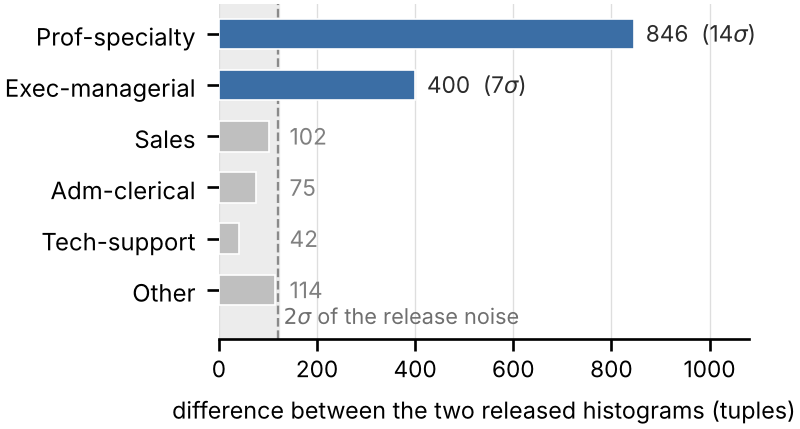
\includegraphics[width=\linewidth]{figures/released.png}
\caption{What the release leaves of the first explanation of the running example: the per-bin difference between the two noisy histograms of Figure~\ref{fig:candidates}(a). At $2k/\epsilon_H=30$ that difference has standard deviation $60$ per bin. Two bins clear twice it; the other four do not.}
\label{fig:released}
\end{figure}

\paragraph{The algorithms on the running example.}
Take the refinement of Example~\ref{ex:running} on Adult: $N=48{,}842$, $|\views|=1{,}052$, $|\Attrs|=10$, $k=5$, $\lambda=\tfrac12$ and $\epsilon=1$, so each stage receives $1/3$ and Eqs.~\eqref{eq:tau-rule} and~\eqref{eq:gamma-rule} give $\tau=15$ and $\gamma\approx150$.
Algorithm~\ref{alg:main} scores the $1{,}052$ views by $\Use$ and keeps $15$.
The view $\texttt{education}=\texttt{Masters}$ survives on a coverage of $0.068$ and a
representativeness of $0.80$, against the $0.92$ that Eq.~\eqref{eq:rep-upper} allows a view of
its size.
\added{At $\gamma_R=N$ it scored $0.53$, which is that ceiling exactly: the measure read none of
the reference attributes and would have returned $0.53$ whatever they held. The $0.12$ it now
falls short by is the distributional signal Eq.~\eqref{eq:gammaR-rule} leaves in.}

Algorithm~\ref{alg:topk} pairs it with each attribute, and the first round selects \texttt{occupation}, whose two histograms are those of Figure~\ref{fig:candidates}(a).
Figure~\ref{fig:released} shows what survives their release: the explanation is legible exactly where it is large, and the four small bins are returned as noise.
The counter of \texttt{occupation} is then incremented, and with $\lambda=\tfrac12$ every remaining candidate on that attribute is scored at half its value in the next round, which is what moves the second explanation onto a different attribute.

\paragraph{Exactness of the second stage.}
Because $\gamma$ is fixed once and the diversity factor depends only on attributes already released, the score of line~4 is the marginal gain of its candidate in the set objective of Definition~\ref{def:setobj}, so selecting the highest-scoring candidate is one step of greedy on it.
On that objective greedy is not an approximation but exact, because it separates over attribute groups and each group contributes a concave function of how many of its candidates are taken; Proposition~\ref{prop:greedy-exact} in Appendix~\ref{app:greedy} states both halves.
The optimality is over the candidates the view stage admits rather than over $\mathcal{E}$; what the filter discards is the cost Section~\ref{subsec:two-stages} leaves open.
This is what makes a non-private greedy run a usable reference point: with the candidate set and $\gamma$ held fixed it is the optimum, so the gap the private algorithm shows against it is attributable to the mechanism alone.

\subsection{Privacy and Cost}
\label{subsec:dp-proof}

\begin{proposition}[Sensitivity of the released histograms]
\label{prop:histogram-release-sensitivity}
Fix a candidate $(p,A)$ and write $H^j=\hist{Q_j(\pD)}{A}$ for $j=1,2$.
The pair $(H^1,H^2)$ has $L_1$-sensitivity at most $2$, and the difference $H^1-H^2$ has $L_1$-sensitivity at most $1$.
\end{proposition}

\begin{proof}
Since $Q_1$ and $Q_2$ are selections, one added tuple joins at most one bin of $A$, and it may be selected by both queries, by one of them, or by neither.
It therefore changes each of the two histograms in at most one coordinate and by at most $1$, which gives $2$ for the pair.
For the difference, the affected coordinate changes by $d_1-d_2$ with $d_1,d_2\in\{0,1\}$, so by at most $1$, and all other coordinates are unchanged.
\end{proof}

Releasing the pair therefore calls for $\Lap(2k/\epsilon_H)$, as in Algorithm~\ref{alg:topk}; the variant that releases only the difference uses $\Lap(k/\epsilon_H)$ for the same budget.

\begin{proposition}[Privacy of the framework]
\label{thm:alg1-dp}
Algorithm~\ref{alg:topk} satisfies $(\epsilon_S+\epsilon_H)$-differential privacy, and, with $N=|D|$ public as in Proposition~\ref{prop:usefulness-sensitivity}, Algorithm~\ref{alg:main} satisfies $\epsilon$-differential privacy.
\end{proposition}

\begin{proof}
Take Algorithm~\ref{alg:topk} first.
Each round invokes the exponential mechanism with budget $\epsilon_S/k$ on a utility of sensitivity $1/(1+\gamma)$ (Proposition~\ref{prop:selection-utility-sensitivity}), which is $(\epsilon_S/k)$-DP, and the Laplace mechanism with budget $\epsilon_H/k$ on a pair of histograms of $L_1$-sensitivity $2$ (Proposition~\ref{prop:histogram-release-sensitivity}), which is $(\epsilon_H/k)$-DP.
Both calibrations are legitimate because $\gamma$ is a constant of the mechanism rather than a function of the input: by Eq.~\eqref{eq:gamma-rule} it is determined by $k$, $|\views|$, $|\Attrs|$ and the budget, all of which are fixed before the data is read, so the sensitivity bound it induces holds uniformly over all databases.
The rounds are adaptive, since $u_i$ depends on the attributes already selected, but adaptive sequential composition applies~\cite{DBLP:series/synthesis/2016Li} and gives $k(\epsilon_S/k+\epsilon_H/k)=\epsilon_S+\epsilon_H$.
The conditioning covers the candidate set as well as the utility: $C_i$ is fixed by $\widehat{\mathcal{P}}$ and by what has already been released, both of them outputs of earlier steps, so for a fixed history it is the same set on neighbouring databases.

For Algorithm~\ref{alg:main}, view selection is $\epsilon_P$-DP by Theorem~\ref{thm:oneshot-topk} together with the sensitivity $\added{4/|D|}$ of Proposition~\ref{prop:usefulness-sensitivity}, which the algorithm passes to the mechanism.
This is the one place the hypothesis on $N$ is used, and it is used for the calibration rather than for the bound: Proposition~\ref{prop:usefulness-sensitivity} already covers neighbours of different sizes, but the theorem being invoked compares a \emph{single} mechanism on two inputs, and a $\Delta$ recomputed from each input would make the runs on $D$ and on $D'$ two different mechanisms.
\added{Fixing $\Delta=4/\bar N$ from a public $\bar N\le|D|$ that does not depend on $D$ removes that.}
Candidate construction is post-processing.
Sequential composition over the two stages gives $\epsilon_P+\epsilon_S+\epsilon_H=\epsilon$, so the pipeline as a whole is $\epsilon$-differentially private.
\end{proof}

\paragraph{Complexity.}
\label{subsec:complexity-analysis}
Let $|\mathcal{P}|$ be the number of candidate views, $a=|\Attrs|$ the number of explanation attributes, $r=|\mathcal{A}_R|$ the number of reference attributes, $b$ the maximum number of bins per attribute, and $N=|D|$.
Computing $\Use$ for every view costs $O(|\mathcal{P}|\,r\,N)$ by the direct route of one pass over $D$ per view, since $\Rep_{\gamma_R}$ averages over the reference attributes and every view needs its own histogram on each of them; the one-shot top-$\tau$ mechanism adds $O(|\mathcal{P}|\log\tau)$, one Gumbel draw per view and a heap of size $\tau$.
Materialising the bin vectors of the $\tau$ retained views over the $a$ explanation attributes costs $O(\tau a N)$.
Scoring is then paid once rather than once per round.
Because $\gamma$ is fixed by Eq.~\eqref{eq:gamma-rule}, $\HD_\gamma(p,A)$ is the same number in every round, so the $\tau a$ values are computed once in $O(\tau a b)$; a round only rescales each of them by its diversity factor, samples, and perturbs the two histograms of the winner, which is $O(\tau a+b)$.
The total is
\[
O\!\left(|\mathcal{P}|\,r\,N + \tau a\, N + \tau a b + k(\tau a + b)\right)
= O\!\left(\big(|\mathcal{P}|\,r + \tau a\big)N\right),
\]
because $b\le N$ and $k\le N$.
The two data passes therefore absorb everything else, and the $k$ selection rounds, the only part that spends privacy budget, cost $O(k(\tau a+b))$ and are independent of $N$.
Of the two passes only the first is independent of $k$ as well as of $\epsilon$; the second carries $\tau=\min(3k,|\mathcal{P}|)$.


